\lecture{8}{2025-03-14}{Arithmetic circuit}{}

\subsection{Adders}
\begin{parag}{Adders of two 1-bit binary}
Let us start from the simplest binary addition of one bit. The resulting sum is at most on two bits:
\begin{itemize}
    \item The rightmost bit is called $sum$(s)
    \item The leftmost bit is called $carry(c)$; it is produced as a carry-out when being a both bits being added are logical one
\end{itemize}
The goal is to create an addition with boolean arithmetic. Let us create a truth table:
\begin{center}
    \begin{tabular}{cccc}
        $x$ & $y$ & $s$ sum & $c$ carry \\
        \hline
        0 & 0 &0&0 \\
        0 & 1 & 1 & 0\\
        1 &0 &1&0\\
        1&1&0&1
\end{tabular}
\end{center}
we can as seen here, use one expression when the output is $1$ for the sum and another when the output is $1$ for the carry:
\begin{align*}
    s = \overline{x}y + x \overline{y} = x \oplus x
\end{align*}
For the carry:
\begin{align*}
    c = xy
\end{align*}

Which gives us the digital logic circuit:
\begin{center}
    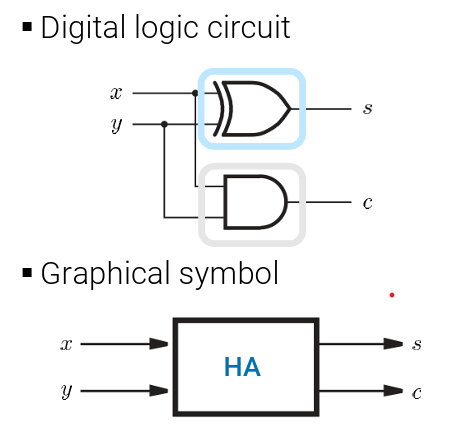
\includegraphics[scale=0.7]{12025-03-14.png}
\end{center}


\end{parag}
\begin{parag}{Addition of two $n$ bit binary number}
    A binary $n$-bit adder has two operands $0 \leq x, y \leq 2^n - 1$ and a carry in $c_{in} \in \{0 1\}$ as inputs, and produces as outputs:
    \begin{itemize}
        \item sum $0 \leq s \leq 2^n -1$
        \item Carry out $c_{out} \in \{0, 1\}$ such that:
            \begin{align*}
                x +  y + c_{in} = 2^nc_{out} + s
            \end{align*}
    \end{itemize}
    The solution to the above equation is:
    \begin{align*}
        s = (x + y + c_{in}) \mod 2^n
    \end{align*}

    Then we get for the carry:
    \begin{align*}
        c_{out} = \begin{cases}
            1 \text{ if } (x + y + c_{in}) \geq 2^n \\
            0 \text{ otherwise }
        \end{cases}
        = \lfloor  \frac{x + y + c_{in}}{2^n}\rfloor
    \end{align*}
    It is \important{impractical} to start from the truth table for $n$bit addition.
\end{parag}
\begin{parag}{Iterative approach}
    For the iterative algorithm:
    \begin{itemize}
        \item Add each pair of bits at the position $i, o \leq i \leq n$
        \item The addition at the bit position $i$ needs to include a carry-in at the position $i$ (i.e., carry out from the position $i-1$); it also generates a carry-in for the position $i + 1$
    \end{itemize}
    The $1$ bit adder reduces to a primitive module called \important{full-adder (FA)} with three binary inputs and two binary outputs such that:
    \begin{align*}
        x_i + y_i + c_i = 2c_{i+1} + s_i
    \end{align*}
\end{parag}
\begin{parag}{Full adder:}
    The goal now is to build the truth table for those outputs $s_i$ and $c_{i+1}$ from $x_i, y_i, c_i$:
    \begin{center}
    \begin{tabular}{ccccc}
        $x_i$ & $y_i$ & $c_i$ & $s_i$ & $c_{i+1}$ \\
        \hline
        0 & 0 & 0&0&0 \\
        0&0&1&1&0\\
        0&1&0&1&0\\
        0&1&1&0&1\\
        1&0&0&1&0\\
        1&0&1&0&1\\
        1&1&0&0&1\\
        1&1&1&1&1
    \end{tabular}
    \end{center}
    
    With the logical expression:
    \begin{align*}
        s_i &= \overline{x_i} \overline{y_i}c_i + \overline{x_i}y_i \overline{c_i} + x_i \overline{y_i} \overline{c_i} + x_iy_ic_i \\
            &= (x_iy_i + \overline{x_i} \overline{y_i})c_i + ( \overline{c_i}y_i + x_i \overline{y_i}) \overline{c_i} \\
            &= \overline{(x_i \oplus y_i)} c_i + (x_i \oplus y_i) \overline{c_i} = x_i \oplus y_i \oplus c_i
    \end{align*}
    And for $c_{i+1}$:
    \begin{align*}
        c_{i+1} &= \overline{x_i}y_ic_i + x_i \overline{y_i}c_i + x_iy_i \overline{c_i} + x_iy_ic_i \\
                &= ( \overline{x_i}y_i + x_i \overline{y_i})c_i + x_iy_i( \overline{c_i} + c_i) \\
                &= (x_i \oplus y_i)c_i + x_iy_i
    \end{align*}
    With give us:
    \begin{align*}
        c_{i+1} = x_iy_i + x_ic_i + y_ic_i
    \end{align*}
    \begin{subparag}{Example}
        Let us create a full-adder from a half adders:\\
        \begin{itemize}
            \item Half adder:
                \begin{align*}
                    s = \overline{x}y + x \overline{y} = x \oplus y\\
                    c = xy
                \end{align*}
            \item Full adder:
                \begin{align*}
                    s_i = x_i \oplus y_i \oplus c_i\\
                    c_{i+1} = (x_i \oplus y_i)c_i + x_iy_i
                \end{align*}
        \end{itemize}

        \begin{center}
            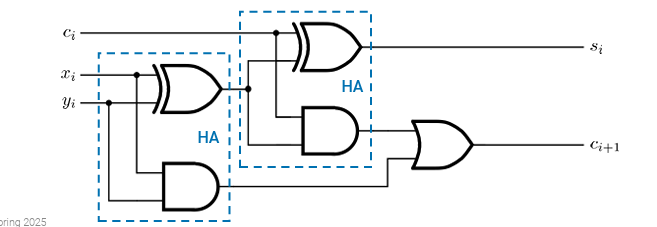
\includegraphics[scale=0.7]{22025-03-14.png}
        \end{center}
        Here we see the first result with the left \important{HA} and then go into a xor to the other adder
    \end{subparag}

    \begin{subparag}{Full adder}
        Here the logical circuit to the final logic expression:
        \begin{align*}
            s_i = x_i \oplus y_i \oplus c_i \\
            c_{i+1} = x_iy_i + x_ic_i + y_ic_i
        \end{align*}
        is:
        \begin{center}
            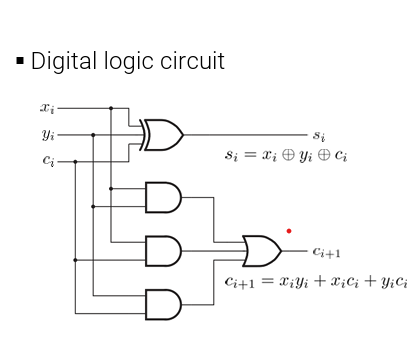
\includegraphics[scale=0.5]{32025-03-14.png}
        \end{center}
    With the graphical symbol     
        \begin{center}
            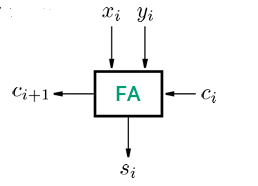
\includegraphics[scale=1.1]{42025-03-14.png}
        \end{center}
   \end{subparag}
   And the to be able to do an addition:
   \begin{itemize}
       \item Starting from the least significant digit, we add pairs of digits, progressing to the most significant digit
       \item Carry "ripples" through the adder stages
   \end{itemize}
   \begin{framedremark}
       There will be the same schema for the substraction juste below but I didn't put it here again to save the picture to document ratio. (but it is the slide 15)
   \end{framedremark}
   
\end{parag}
\begin{parag}{Substraction of two $1$ bit binary number}
    Subtraction generates two bits:
    \begin{itemize}
        \item \important{difference} (d), the result of the subtraction
        \item \important{borrow} (b), produced as a borrow out when the subtrahend is larger than minend
    \end{itemize}
\end{parag}
\begin{parag}{Subtraction of two n-bit unsigned number}
    it is \important{impractical} to start from the truth tables for $n$ bit substraction, if the exact same approach as the addition:
    \begin{itemize}
        \item Substract each pair of bits at the position $i, o \leq i < n$
        \item Subtraction at the bit position $i$ needs to include a borrow in at position $i$ (i.e., borrow out from the position $i - 1$); it also generates a borrow in position $i + 1$
    \end{itemize}

\end{parag}
\begin{parag}{Full subtractor}
    from the truth table:
    \begin{center}
    \begin{tabular}{ccccc}
        $x_i$ & $y_i$ & $b_i$ & $d_i$ & $b_{i+1}$ \\
        0&0&0&0&0\\
        0&0&1&1&1\\
        0&1&0&1&1\\
        0&1&1&0&1\\
        1&0&0&1&0\\
        1&0&1&0&0\\
        1&1&0&0&0\\
        1&1&1&1&1
    \end{tabular}
    \end{center}
   Which gives us:
   \begin{align*}
       d_i &= \overline{x_i} \overline{y_i} b_i + \overline{x_i}y_i \overline{b}_i + x_i \overline{y_i} \overline{b_i} + x_iy_ib_i\\
           &= ( \overline{x_i} \overline{y_i} + x_iy_i)b_i + ( \overline{x_i}y_i + x_i \overline{y_i}) \overline{b_i} = \overline{(x_i\oplus \overline{y_i})}b_i + (x_i \oplus y_i) \overline{b_i}\\
           &= x_i \oplus y_i \oplus b_i
   \end{align*}
   \begin{align*}
       b_{i+1} &= \overline{x_i} \overline{y_i} b_i + \overline{x_i}y_i \overline{b_i} + \overline{x_i}y_i \overline{b_i} + \overline{x_i}y_ib_i + x_iy_ib_i \\
    &= ( \overline{x_i} \overline{y_i} b_i + \overline{x_i}y_ib_i) + ( \overline{x_i}y_i \overline{b_i} + \overline{x_i}y_ib_i) + ( \overline{x_i}y_ib_i + x_iy_ib_i) \\
    &= \overline{x_i}b_i + \overline{x_i}y_i + y_ib_i
   \end{align*}
   With the same principle to the $n$bit ripple carry subtractor:
\begin{center}
    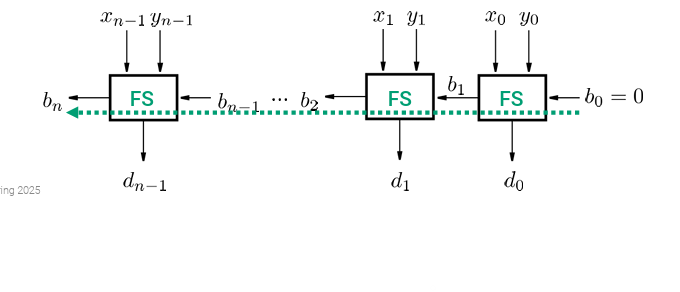
\includegraphics[scale=0.8]{52025-03-14.png}
\end{center}

   
   
\end{parag}
\begin{parag}{Adders-Subtractors in two's complement}
    Recall that subtracting two numbers in two's complement format requires using the two's complement of one operand:
    \begin{align*}
        X - Y = X + \overline{Y} + 1
    \end{align*}
    where 
    \begin{itemize}
        \item $ \overline{Y}$ is obtained by complementing every bit of $Y$
        \item Assume a control signal $op$ determines which $op$eration to perfom ( $op = 0$ is addition and $op = 1$ is subtraction)
    \end{itemize}
If we now assume a control signal $op$ determines which operation to perform then we can create the function $f$:
\begin{align*}
    f ( X, Y) = \begin{cases}
        X + Y \text{ if } op = 0\\
        X + \overline{Y} + 1, \text{ otherwise}
    \end{cases}
\end{align*}

Which with some  boolean algebraic operations:
\begin{align*}
    f(X, Y) &= \overline{op}(X + Y) + op(X + \overline{Y} + 1) \\
            &= ( \overline{op} + op) X + \overline{op}Y + op \overline{Y} + op \\
            &= X + \overline{op}Y + op \overline{Y} + op \\
            &= X op \oplus Y + op
\end{align*}

\begin{center}
    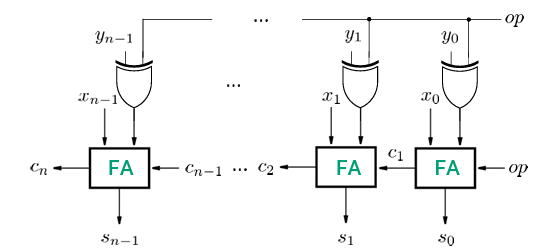
\includegraphics[scale=0.7]{62025-03-14.png}
    
\end{center}


\end{parag}

\subsection{Fast Adders}
\begin{parag}{Performance Matters}
Addition and subtraction are fundamental operations performed frequently. How quickly a result can be produced greatly impacts the system's performance. The performance is determined by the worst case delay.\\
The system's value is measured as a ratio:
\begin{align*}
    value = \frac{performance}{price}
\end{align*}
\begin{subparag}{Example}
    For example if we take the full adder (see the circuit there), There is a delay for each of the sum and the carry out, therefore for the worst case delay, we get:
    \begin{align*}
        t_{max} &= \text{max}(t(s_i), t(c_{i+1}))\\
                &= \text{max}(2t(XOR), t(XOR) + t(AND) + t(OR) \\
                &= 3 \text{ Gate Delays}
    \end{align*}

    
    
\end{subparag}
\end{parag}

\subsection{Shifting}
\begin{parag}{Barrel shifter}
    \begin{definition}
        A \important{barrel shifter} is a combinational logic circuit with $n$ data inputs $n$ data outputs, and a set of control inputs that specify how to shift data between the input and the output
    \end{definition}
    A barrel shifter inside a processor can typically specify
    \begin{itemize}
        \item \important{direction} of shift (left, right)
        \item \important{type} of shift (logical, arithmetic, circular/rotation)
        \item \important{amount} of shift (typically $0$ to $n-1$ bits)
    \end{itemize}
    implemented as a sequence of multiplexers (MUX), each shifting their input by twice as many positions as the previous MUX.
\begin{subparag}{How it works}
    A shifting is like you could imagine with only all bits going left or right and $0$ \textit{"replacing"} the one that get crushed.
\end{subparag}
\end{parag}


















